\titreTD{\thenumTD}{Recouvrements entre Orbitales Atomiques}
%%%%%%%%%%%%%%%%%%%
%##########################################################################
% OM pour d\'ecrire la liaison chimique
%##########################################################################
\textit{Pour se pr\'eparer \`a ces exercices, on pourra rappeler les sch\'emas des orbitales s, $p_x$, $p_y$, $p_z$ selon un rep\`ere impos\'e}.

\exo{Recouvrement d'orbitales atomiques}
Dans une mol\'ecule A$-$B, on \'etudie le recouvrement entre 2 orbitales atomiques, l'une centr\'ee sur un atome A, l'autre sur  B. Pour l'ensemble de cet exercice, les axes sont d\'efinis selon la figure du rep\`ere ci-dessous (l'axe internucl\'eaire d\'efinit l'axe Oz, et $x$ est dans le plan de la feuille, vers le haut). 
\\

Pour chaque cas propos\'e,

\begin{minipage}[c]{0.8\linewidth}
\begin{enumerate}[(i)] 
\item dessinez les orbitales en pr\'esence
\item indiquez la nature du recouvrement : $\sigma$, $\pi$ ou nul 
\item  pr\'ecisez s'il s'agit d'un recouvrement positif, n\'egatif ou nul
\end{enumerate} 
\end{minipage}
\begin{minipage}[l]{0.1\linewidth}     
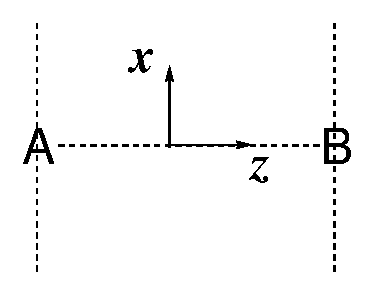
\includegraphics[scale=0.4]{figure/AB_repere.eps}\\   
Rep\`ere
\end{minipage}

\vspace{0.3cm}

\begin{minipage}[c]{0.5\linewidth}
\begin{enumerate}[\bf 1)]
\item $+2p_{x\textsc{a}}\ \, |+\,2p_{x\textsc{b}}$ 
\item $+2p_{z\textsc{a}}\ \, |-\,2p_{z\textsc{b}}$ 
\item $\ \, +2s_\textsc{a}\ \, |+\,2s_\textsc{b}$ 
\item $\ \, +2s_\textsc{a}\ \, |+\,2p_{z\textsc{b}}$ 
\item $+2p_{x\textsc{a}}\ \, |+\,2s_\textsc{b}$ 
%\item $+3p_{y\textsc{a}}\ \, |-\,3p_{y\textsc{b}}$
%\item $-3p_{x\textsc{a}}\ \, |-\,3s_\textsc{b}$
%\item $-2p_{x\textsc{a}}\ \, |-\,3p_{x\textsc{b}}$
\end{enumerate} 
\end{minipage} \hfill
\begin{minipage}[c]{0.5\linewidth}
 \textbf{Exemple :}  $+2s_\textsc{a}\ |-\,2s_\textsc{b}$
\begin{enumerate}[~~(i)] 
\item    Dessin~:\\[-0.3cm] 

   \  \  \  \  \   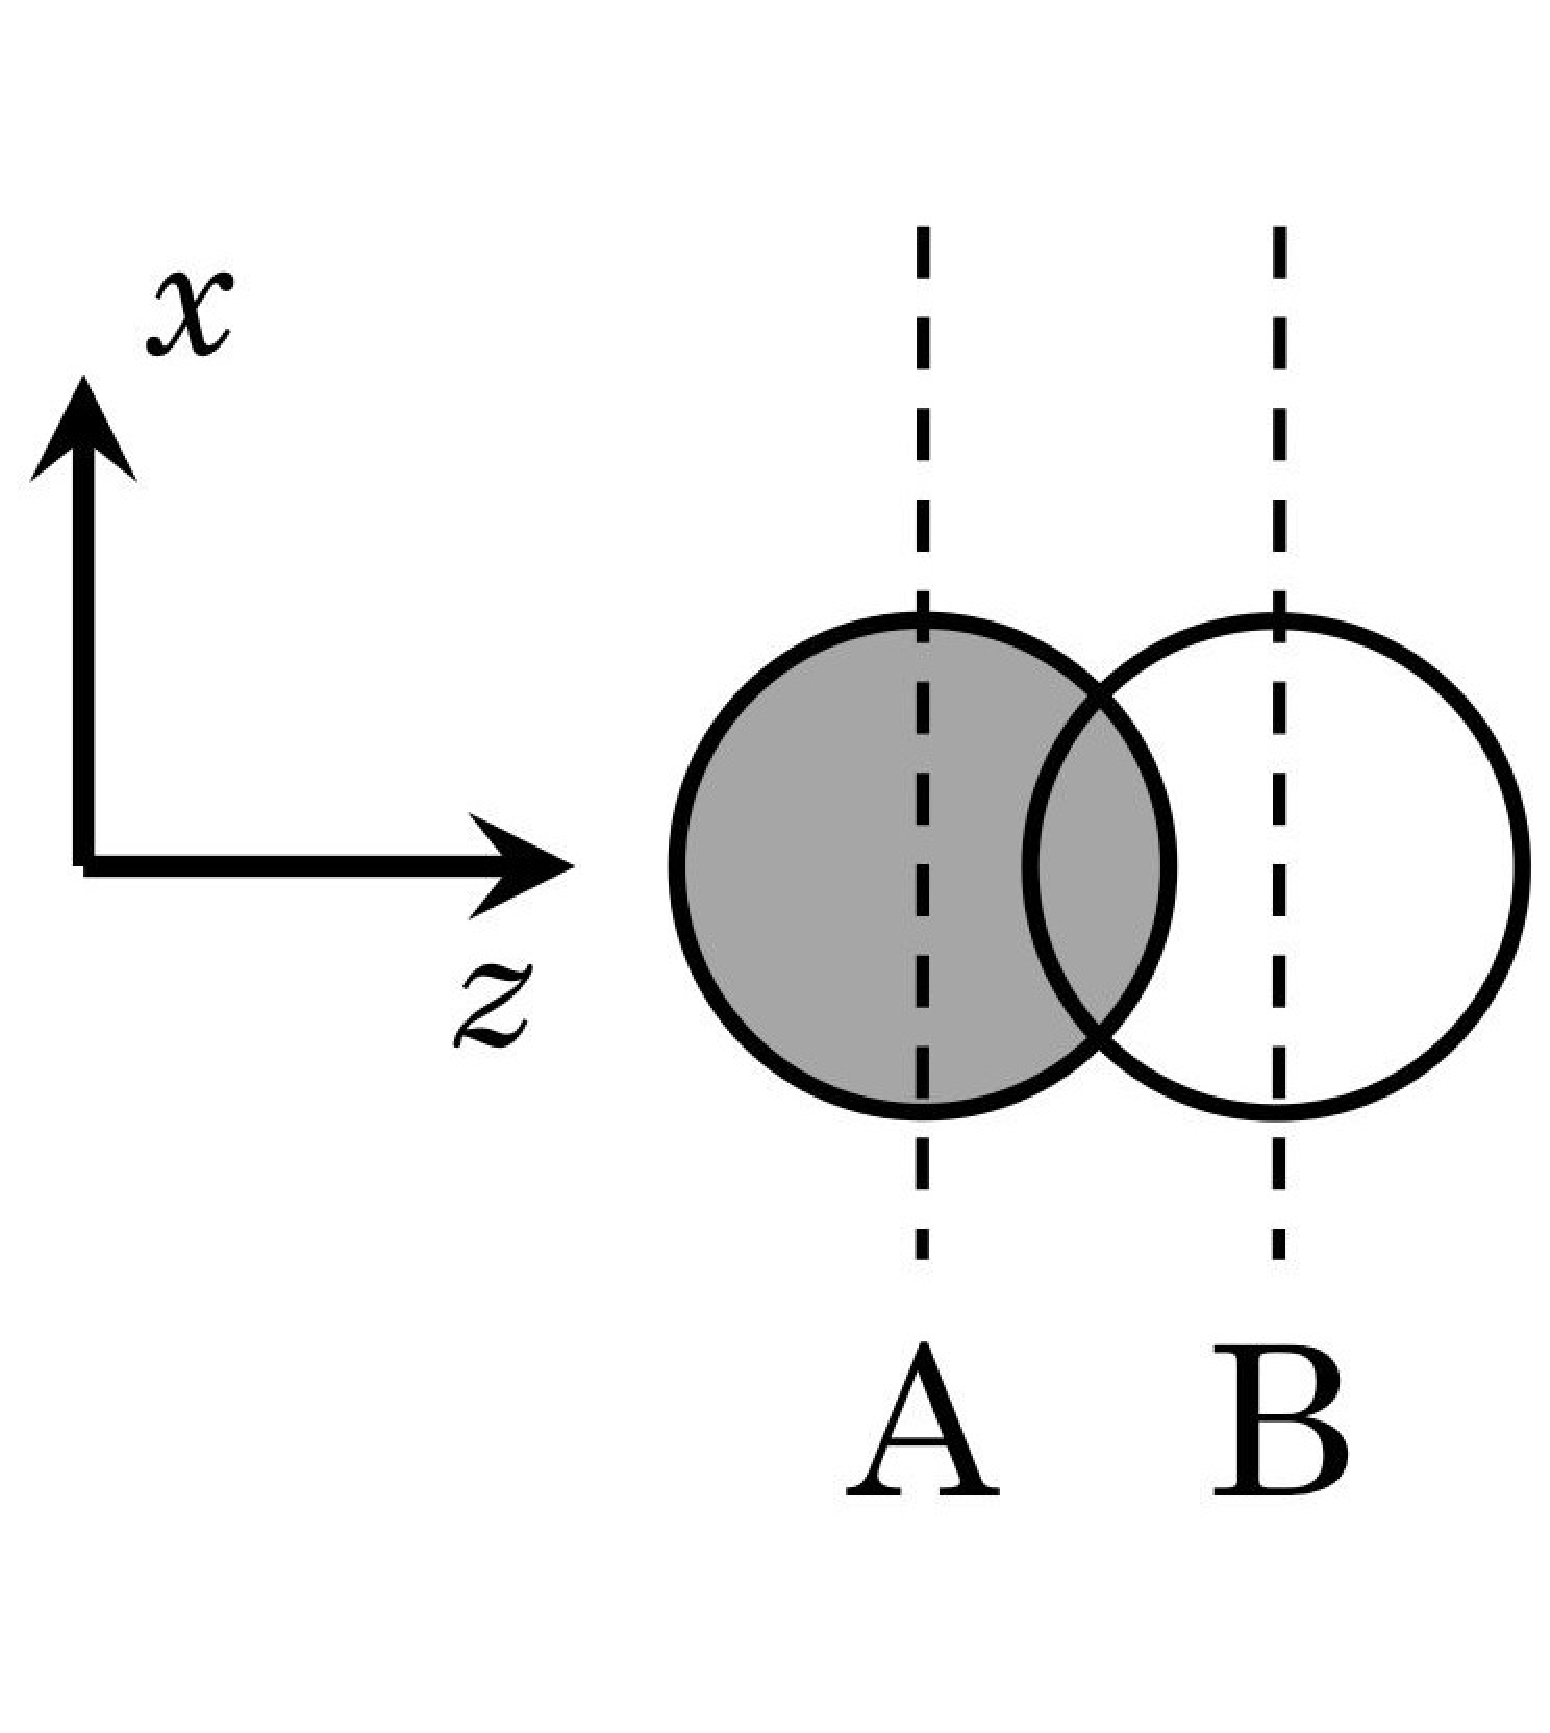
\includegraphics[scale=0.09]{figure/interactionOA.eps}
\item       Recouvrement axial, donc $\sigma$
\item       Recouvrement <0 car de phase $\neq $
\end{enumerate} 
\end{minipage}

%--------------------------------------------------------------------------
\exo{D\'efinition}
\begin{enumerate}[\bf 1)]
\item   Rappelez l'expression du recouvrement $S_{ab}$, entre une orbitale $ \Psi_a(r,\theta,\phi)$, et  $\Psi_b(r,\theta,\phi)$.
\item  Que vaut exactement cette int\'egrale si $ \Psi_a(r,\theta,\phi)=\Psi_b(r,\theta,\phi)=\Psi(r,\theta,\phi)$.
\end{enumerate} 
%--------------------------------------------------------------------------
\exo{Sur un m\^eme atome, les orbitales ne se recouvrent pas}

\begin{enumerate}[\bf 1)]
\item    Montrez graphiquement que les orbitales $2s_A$ et $2p_{z_{A}}$ (centr\'ee sur le m\^eme atome A), ont un recouvrement nul. Expliquez.
\item    A quoi correspond la combinaison  $2s_A+2p_{z_{A}}$~? 
\end{enumerate} %\exo{Variation du Recouvrement avec la distance}
%--------------------------------------------------------------------------
